The terminator T-2000 is a science-fiction spectacle of a robot -- until you see the price. Channeling the inspiration many high school students may have for robotics, MEIOSIS robotics aims to provide an affordable manipulator to educators and enthusiasts. MEIOSIS uses primarily 3-D printed components and easily accessible materials. Among these materials are a Raspberry PI, smart servos and metal tubing. These features create an open-source manipulator accessible to the public to further robotics education.
\hiddensubsection{Physical System Overview}
The physical design of the robotic manipulator is shown in Figures \emph{\ref{fig:overall}, \ref{fig:base}, \ref{fig:link1},} and \emph{\ref{fig:link2}}.

\begin{figure}[htp]
  \centering
  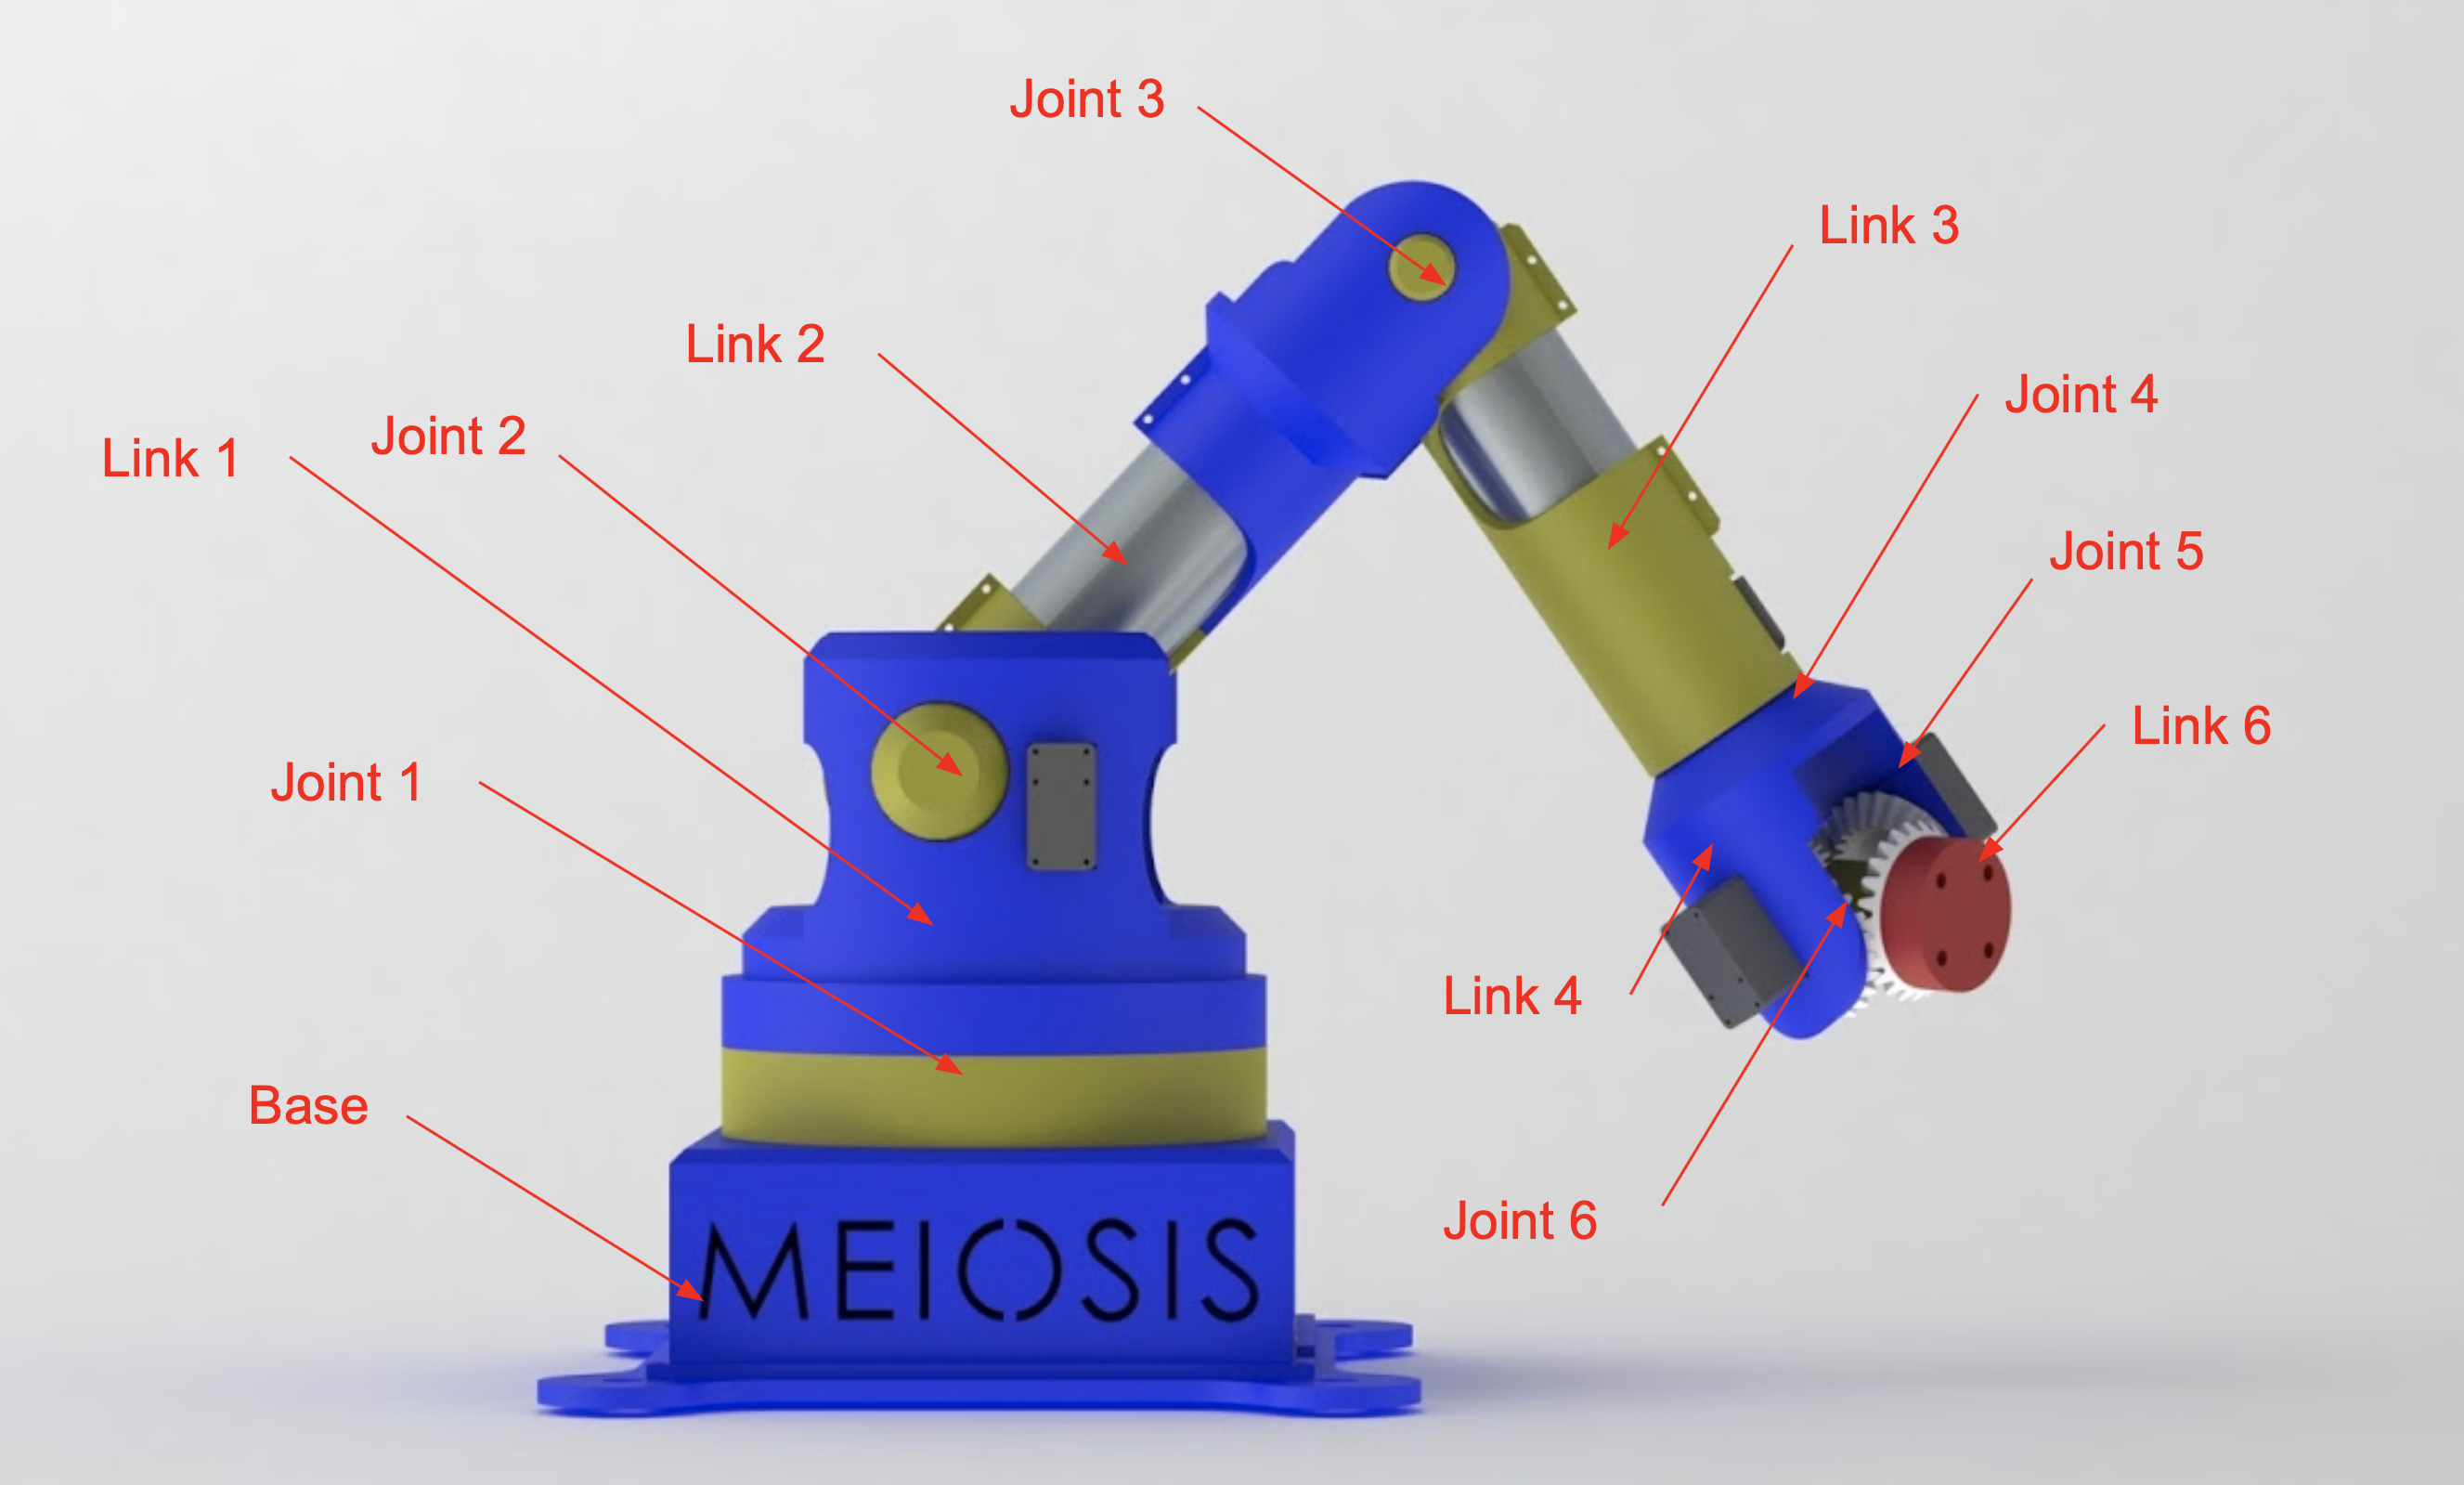
\includegraphics[frame, width=.75\textwidth]{overall_render}
  \caption{Overall System Conceptual Design }
  \label{fig:overall}
\end{figure}

The colored links in \emph{Figure \ref{fig:overall}} distinguish the different joints and links of the manipulator. The overall reach of the robot is 582.5 mm. This length was chosen to decrease material cost and weight while still satisfying requirement 2.1.2 and 2.1.5, allowing the manipulating to pick and place objects to perform basic tasks. The base of the robot is made to contain the Raspberry Pi and other electrical components.
\newpage
\subsubsection{Base}
The base of the manipulator will house several of the electronic components, such as the computational system, power supply, and motor controller. A cross section of the base can be seen in \emph{Figure \ref{fig:base}}.
\begin{figure}[htp]
  \centering
  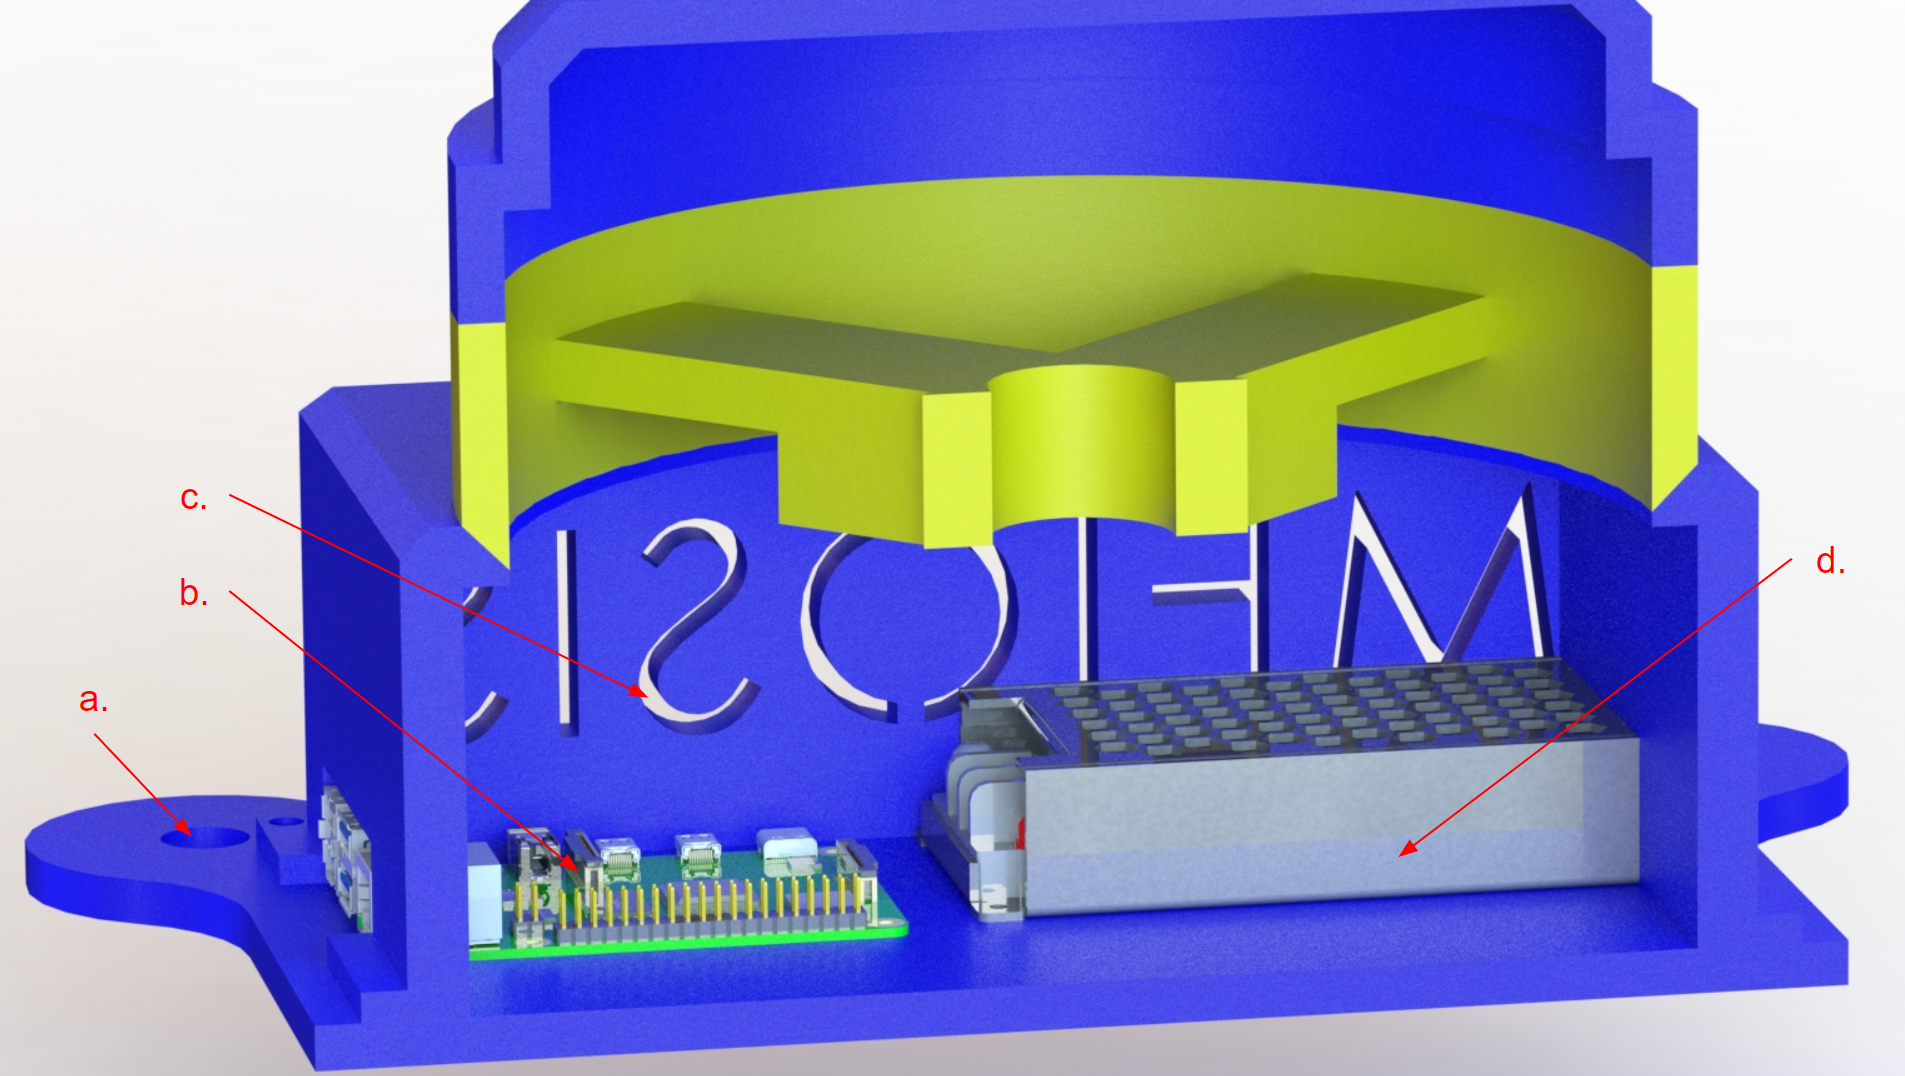
\includegraphics[frame, width=.75\textwidth]{base_callouts}
  \caption{Manipulator Base with Call-outs}
  \label{fig:base}
\end{figure}

From \emph{Figure \ref{fig:base}},
\begin{enumerate}[label=\alph*.]
  \item \emph{Base Supports:}
  The base supports are located at each corner of the base and allow the base of the manipulator to be securely attached to a variety of surfaces with either standard fasteners or suction cups.
  \item \emph{Computational System:}
  The computational system is a Raspberry Pi; it is housed in the base, which allows the Raspberry Pi to be more easily accessible. The primary reason for this system being chosen is to fulfill the budget requirement, 2.1.1. The Raspberry Pi computes the manipulator's inverse kinematics and sends the angle commands to the servos.
  \item \emph{Airflow Cutouts:}
  The side of the base hsd cutouts to allow for airflow through the base; since the power supply is housed inside of the base as well as the computational system, the temperature must be regulated to prevent overheating.
  \item \emph{Power Supply:}
  The power supply is housed in the base as well, which allows the power supply to be more accessible and therefore more modifiable, so the end-user can easily expand the system to fulfill their needs.
\end{enumerate}
\newpage
\subsubsection{Links}
\emph{Figure \ref{fig:link1}} shows the links and their key features.\\
\begin{figure}[htp]
  \centering
  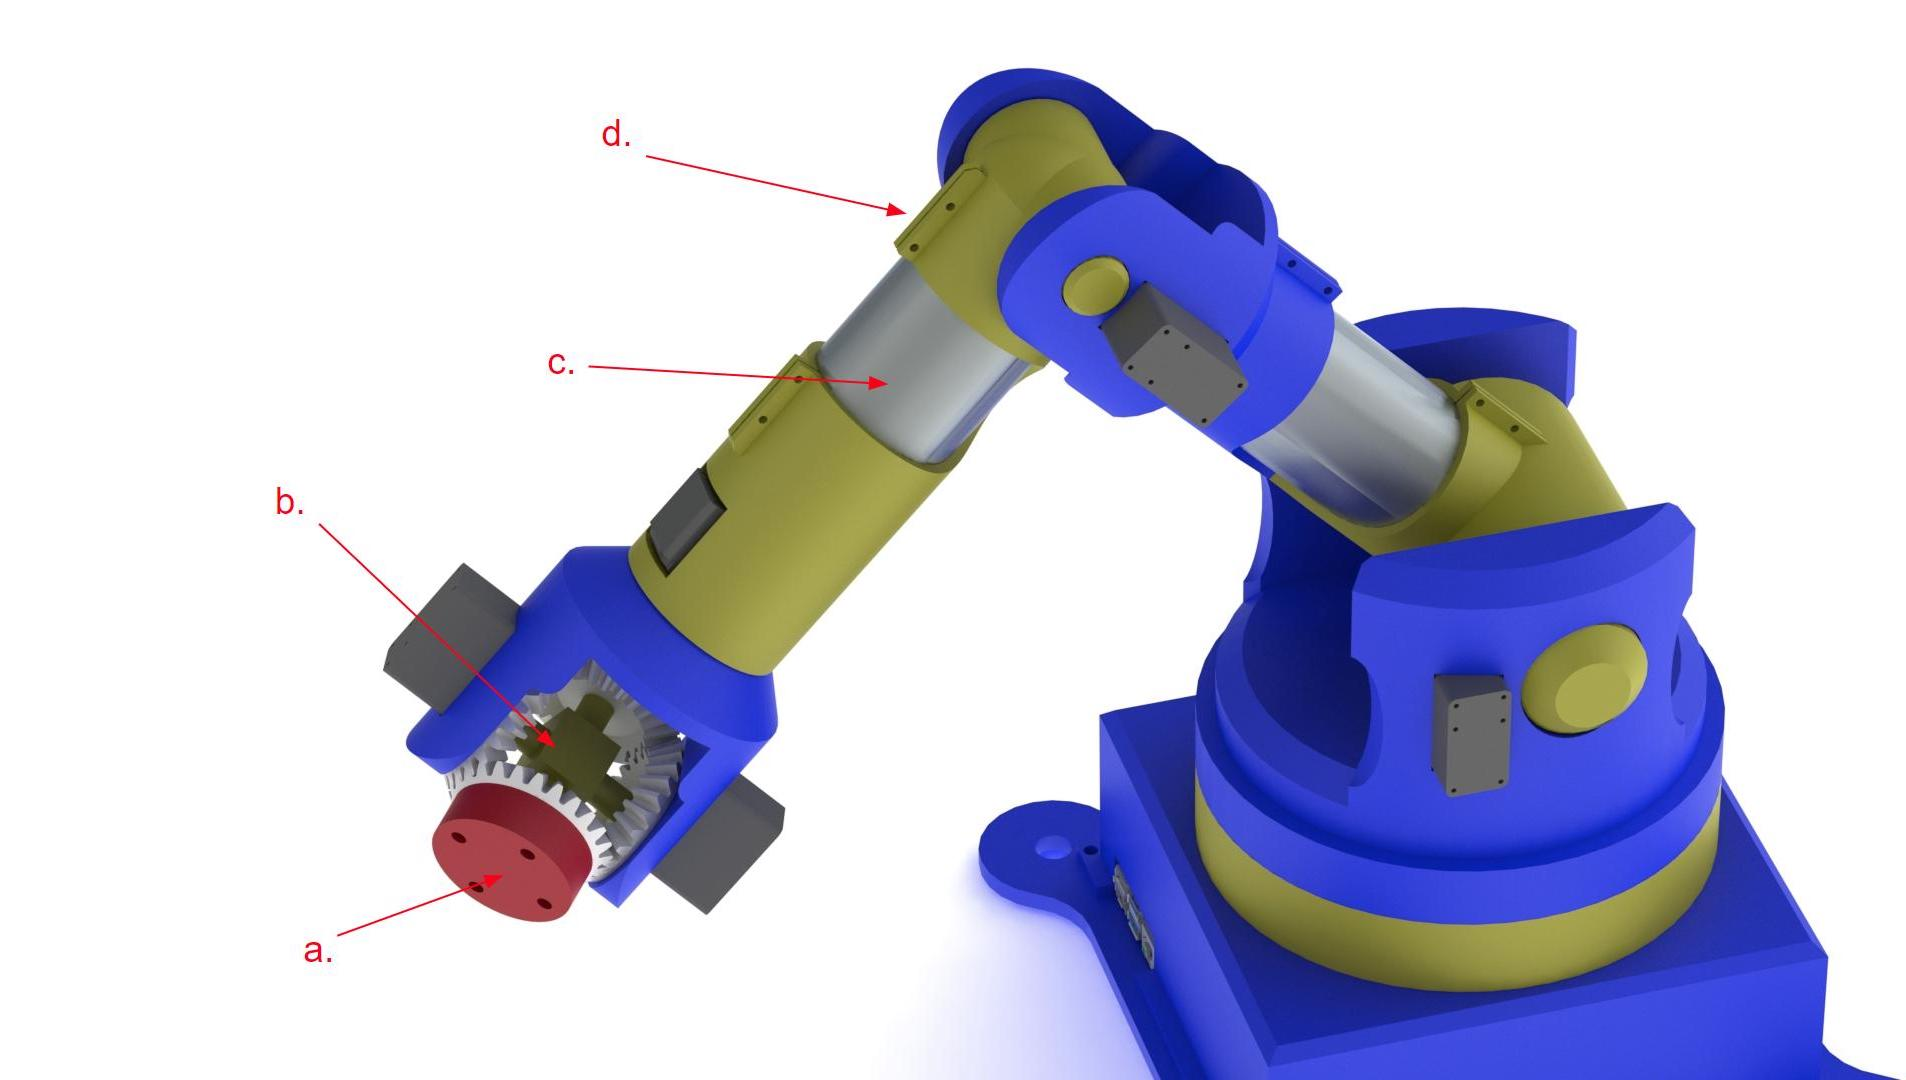
\includegraphics[frame,width=.63\textwidth]{link_callouts}
  \caption{Drawing Showing Key Features of Design}
  \label{fig:link1}
\end{figure} \\
In \emph{Figure \ref{fig:link1}}, call-out (a) shows the connection point for the end effector. The mounting layout is the standard used by the Sawyer manipulator. The end effector mounting layout may be adjusted to accommodate lower cost, more accessible end effectors. Call-out (b) shows the differential gearbox that is used in the manipulator’s wrist, saving space and weight. The manipulator has aluminum tubing as support in the links (c) and are attached to the 3D printed portion of the robot using clamp joints (d) tightened by screws.

\emph{Figure \ref{fig:link2}} depicts the cross section of link 2 for the manipulator.
\begin{figure}[htp]
  \centering
  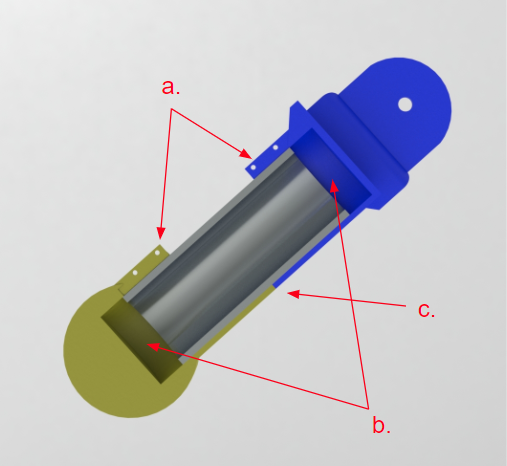
\includegraphics[frame,width=.35\textwidth]{link_cross_section}
  \caption{Drawing Showing Link Cross Section}
  \label{fig:link2}
\end{figure}

The cross section seen in \emph{Figure \ref{fig:link2}} shows the internal design for links two and three. It features two clamps that hold a hollow aluminum bar in place (a) and allows for gaps between the aluminum tube and the 3D printed call-out (b). The proper length is dictated by the 3D printed guides lining up at call-out (c). This design allows for imprecision in the manufacturing of the aluminum tube.

\hiddensubsection{System Functions}
The system can be divided into two subsystems: the electrical and software systems. The electrical subsystem includes the wiring and hardware computational components, power system, actuators with drivers, and sensors. The software subsystem includes the algorithm for the computational system.
\hiddensubsection{Electrical}
\emph{Figure \ref{fig:eblock}} is the block diagram for the electrical system of the manipulator.

\begin{figure}[htp]
  \centering
  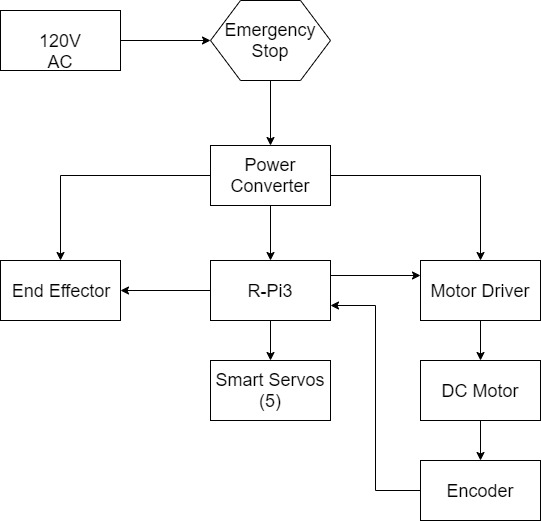
\includegraphics[width=.55\textwidth]{eblock}
  \caption{Electrical System Block Diagram}
  \label{fig:eblock}
\end{figure}

\emph{Figure \ref{fig:eblock}} shows that the electrical systems of the manipulator consists of three main components: the power supply, the Raspberry Pi, and the servos. Power is supplied by the 120V AC from standard wall outlets. A power supply converts the AC voltage to the required voltages for each component. One component is the Raspberry Pi, which performs calculations for motor control. The Raspberry Pi sends signals to the DC motor driver and the five smart servos. The smart servos have an on-board controller, so no feedback will be necessary. However, the first joint, between the base and the first link, is actuated by a DC motor with an encoder to minimize cost.

\hiddensubsection{Software}
\emph{Figure \ref{fig:sblock}} shows the software flowchart for the system.
\begin{figure}[ht]
  \centering
  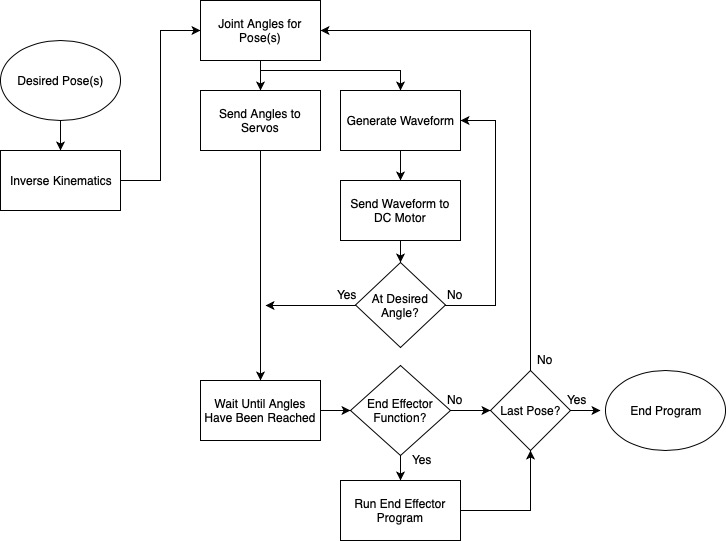
\includegraphics[width=.85\textwidth]{sblock}
  \caption{Software Flowchart}
  \label{fig:sblock}
\end{figure}

\emph{Figure \ref{fig:sblock}} shows that the software receives the desired pose or poses that the user would like the manipulator to reach. Next, the Raspberry Pi uses inverse kinematics to calculate the necessary joint angles. The wave-forms/desired angles are sent to the respective drivers/motors, and positional information is be sent back to the Raspberry Pi to adjust the DC motor angle. When the motors have reached their desired pose, the Raspberry Pi actuates the end effector if it is specified by the user. The system then checks to see if there are any more poses to reach and either repeats the steps in the motor control section given the desired angles of the new pose or ends the program if the last pose has been reached.

\hiddensubsection{Decision Matrices}

Each team member’s conceptual design provides a variety of different options for select issues, and in order to narrow down the options into the best choice decision matrices are used to make unobjective decisions about each individual topic. The weights of each criteria are defined by the average of our votes on how important the criteria is on a scale of one to ten. The same method is used to rate the different options on each criteria. The most important decision that needs to be made is what configuration the manipulator will have as the configuration has an affect on almost all the design choices. There are five potential configurations, and the scores of each option can be seen in \emph{Table \ref{table:manip}}.

\begin{table}[htp]
  \center
  \caption{Configuration Decision Matrix}
  \label{table:manip}
\begin{tabular}{C{3cm}|c@{\hskip 3pt}C{2.5cm}C{2cm}@{\hskip 3pt}C{2cm}@{\hskip 3pt}C{3cm}@{\hskip 3pt}c@{\hskip 3pt}}
\multirow{2}{*}{\textbf{Configuration}} & \multirow{2}{*}{\textbf{Cost}} & \textbf{Educational Value} & \textbf{Ease of Use} &
\textbf{Ease to Program} & \textbf{Ease of Manufacture} & \multirow{2}{*}{\textbf{Total}} \\
\textbf{Weighting} & 10 & 8 & 7 & 2 & 6 & \\\hline
Cartesian w/ Spherical Wrist & \multirow{2}{*}{5} & \multirow{2}{*}{9} & \multirow{2}{*}{10} & \multirow{2}{*}{8} & \multirow{2}{*}{4} & \multirow{2}{*}{232} \\
RRR w/ Spherical Wrist & \multirow{2}{*}{8} & \multirow{2}{*}{9} & \multirow{2}{*}{7} & \multirow{2}{*}{7} & \multirow{2}{*}{8} & \multirow{2}{*}{\textbf{263}} \\
Cylindrical & 7 & 10 & 7 & 8 & 7 & 257 \\
SCARA & 6 & 9 & 8 & 8 & 6 & 240 \\
Spherical & 7 & 10 & 7 & 7 & 6 & 249 \\
\end{tabular}
\end{table}

The results from \emph{Table \ref{table:manip}} show that the solely rotational configuration is the best option, followed closely by the cylindrical. Having translational joints is too be problematic for manufacturing and more expensive, and that is enough of an issue that the rotational manipulator has the advantage over the rest of the options.

Another design choice that needs to be made is what material the manipulator will be constructed out of. The main choices are to 3D print everything, manufacture the manipulator out of aluminum, or use a combination of the two. Cost and accessibility are the two highest weighted criteria as we deem them to be the most important aspects, followed by weight and manufacturability. Durability has the lowest weight because the manipulator should not have enough forces acting on it so that the strength of PLA compared to aluminum should not necessarily affect the manipulator. The grades of each material are shown in \emph{Table \ref{table:mat}}.

\begin{table}[htp]
  \center
  \caption{Material Choice Decision Matrix}
  \label{table:mat}
\small\begin{tabular}{c|cccccc}
\textbf{Material} & \textbf{Cost} & \textbf{Weight} & \textbf{Accessibility} & \textbf{Manufacturability} & \textbf{Durability} & \textbf{Total} \\\normalsize
Weighting & 9.2 & 6.6 & 8 & 6.4 & 5.4 & \\\hline
3D Printed & 8 & 9 & 8 & 9.4 & 5 & 284.16 \\
Aluminum & 4 & 5.8 & 5.8 & 6.6 & 9.2 & 213.4 \\
Combination & 8 & 7.8 & 7 & 9 & 9.2 & \textbf{288.36} \\
\end{tabular}
\end{table}

As seen in \emph{Table \ref{table:mat}}, the winning material is a combination of 3D printing and aluminum. The combination allows the manipulator to have 3D printed parts that would be hard to manufacture out of aluminum or that would not necessarily need to be extremely durable, and allows the use of aluminum for the aspects of the manipulator that need to be strong and durable. This option allows for the best aspects of both materials to be utilized.

The internal computing system for the manipulator is another decision that needs to be made, so another decision matrix is used to decide from the six options available. Because the manipulator is intended to be low cost and used by primary education institutions, cost and ease of use are the two highest weighted criteria. Having a lot of capabilities and being able to function independently are factored in, but are deemed of secondary importance which can be seen in \emph{Table \ref{table:comp}}.

\begin{table}[htp]
  \center
  \caption{Computing Choice Decision Matrix}
  \label{table:comp}
\begin{tabular}{c|ccccc}
\textbf{Computing System} & \textbf{Cost} & \textbf{Capabilities} & \textbf{Ease of Use} & \textbf{Independence} & \textbf{Total} \\
Weights & 10 & 4.2 & 7.6 & 4.2 & \\ \hline
RPi & 7.9 & 6 & 9 & 10 & \textbf{214.6} \\
Jetson & 1 & 7 & 7 & 9 & 130.4 \\
RPi + Arduino & 4.8 & 7 & 8 & 10 & 180.2 \\
Arduino & 9 & 4 & 9 & 3 & 187.8 \\
B Black & 1.2 & 7 & 7 & 10 & 136.6 \\
B Green & 5 & 7 & 6 & 9 & 162.8 \\
\end{tabular}
\end{table}

\emph{Table \ref{table:comp}} shows that the Raspberry Pi is the winner by a significant margin, with only the Arduino coming close to it. While the Pi is not the most capable, its cost is very good and its ease of use and ability to independant functionality edge it over the other more capable competition. The arduino is the most cost effective, but its lack of functionality and low independence are detrimental to its score.

One of the other designs that needs to be selected was the way that the end effectors are attached to the end of the manipulator, and the different categories that are used to grade each option are ease of use, manufacturability, and durability, as seen in \emph{Table \ref{table:ee}}.

\begin{table}[htp]
  \center
  \caption{End Effector Attachment Design Decision Matrix}
  \label{table:ee}
\begin{tabular}{C{3.5cm}|cccc}
\textbf{EE Attachment} & \textbf{Ease of Use} & \textbf{Manufacturability} & \textbf{Durability} & \textbf{Total} \\
Weighting & 3.6 & 5 & 7 & \\\hline
Screw Connections & 6.8 & 8.8 & 9.8 & \textbf{137.08} \\
Snap Fit Joint & 8.6 & 5 & 2.2 & 71.36 \\
Threaded End Effector & 6.3 & 5.4 & 7.3 & 100.78 \\
\end{tabular}
\end{table}

From \emph{Table \ref{table:ee}}, the optimal design turns out to be screw connections in the end effector. The snap fit joint would be easier to use, but to create a functional snap fit connection would be difficult and would likely not be too durable. The threaded end effector is difficult to manufacture and not durable as well, so having connections for screw on the end effector is the clear choice.
